\section{Results}
\label{sec:Evaluation}
We collected data from $9$ subjects, each using our instrumented visualization for approximately $50$ minutes on a series of structured and unstructured tasks. We used the collected data to test the validity and effectiveness of collecting eye-tracking data in visualization space in two ways. 
First, we compared the similarity of our algorithm output to human annotation data, with the similarity between human annotations. We found that our results are on average as similar to human annotations as are human annotations similar to each other. Moreover, we conducted this analysis for all three viewed detection algorithms described in sections~\ref{sec:AOIBasedViewedObjectDetection} to~\ref{sec:MehthodsIntelligentAlgorithm} and showed that the AOI based method (section~\ref{sec:AOIBasedViewedObjectDetection}) performs poorly compared to the other two, and that the prediction component (section~\ref{sec:MehthodsIntelligentAlgorithm}) improves detection accuracy by about $4\%$  (Figure~\ref{fig:quantitative}). 
Second, we demonstrate that our instrumentation method can provide relevant information by showing that viewed objects detected by our instrumentation align with the tasks we asked people to do. Moreover, we show that data collected in this was can be useful in analyzing visual behavior for data visualization users.  
The validity of these evaluation choices are discussed in section~\ref{sec:Discussion}.

\subsection{Study Design }

\textbf{Setup: } We used the visualization and data described in section~\ref{sec:Methods}, and a lightweight $60$Hz EyeX eye-tracker from Tobii connected to a 17'' monitor. Subjects were seated approximately $30''$ away from the display. 

\textbf{Subjects:} We collected data from $9$ graduate and undergraduate students with ages ranging between $20$ years and $30$ years. Six of them were male and three were female. Subjects were paid $10$ for their participation. 

\textbf{Protocol:} Subjects were first given a description of the study's purpose and protocol. They were then introduced to our IMDB PivotPaths visualization and asked to perform a few training tasks to help them get accustomed with the visualization. This introductory part lasted approximately $10$ minutes on average. The main section of the study followed, involved multiple instances of four types of tasks, and lasted approximately $50$ minutes. 


\textbf{Tasks:} We asked subjects to complete four types of tasks. We aimed to balance structured tasks and unstructured tasks. To solve the structured tasks, subjects had to consider a set of objects that was better defined and less variable than in unstructured tasks. This made it easier for us to test the degree to which our detection of viewed objects is aligned with the data required to complete the tasks. On the other hand, data collected for unstructured tasks may be better at informing designs of future analysis systems of such data. We limited the time we allowed subjects to spend on each task. This was done for two reasons: to limit the total duration of the study, and to make results comparable across time and users.

\begin{itemize}
	\item \textbf{Task1 (structured):} Finding four commonalities between pairs of movies. The tasks were limited at three minutes each, and subjects solved the following four instances of this task: (i) Raiders of the Lost Ark and Indiana Jones and the Last Crusade; (ii) A and B; (iii) C and D; (iv) E and F.  
	\item \textbf{Task2 (structured):} Ranking collaborations between a director and three actors ($2$ minutes).  Subjects complete the following four task instances: A and B,C,D; 
	\item \textbf{Task4 (semi-structured):} Given three movies, subjects were asked to recommend a fourth ($5$ minutes). Subjects solved three such tasks: 
	\item \textbf{Task5 (unstructured):} Given a brief and incomplete description of the ``Brat Pack'', a group of young actors popular in the 80's, subjects were asked to find additional members and movies they acted in. Subjects solved one such task, in approximately $5$ minutes. 
\end{itemize}

\subsection{Results}
\subsubsection{Data collected automatically is similar to that of human annotators}
\label{sec:EvalResults}

We compared lists of viewed objects produced by our instrumentation to similar lists created manually by human coders who manually inspected screen captures with overlaid gaze positions. To this end, we enlisted the help of five coders and asked them to code data corresponding to one task of approximately three minutes, for six subjects.  Each coder spent approximately one hour on each of the six subjects. Four coders completed all assigned tasks, while one coder was able to code only three of the six data sets. The six subjects were selected randomly and were the same for all four coders. We found that similarities between the results of human coders and the `intelligent' instrumentation described in section~\ref{sec:MehthodsIntelligentAlgorithm} are very close to the similarities between the results of human coders. These results are shown in Figure~\ref{fig:quantitative}, the `intelligent' and `coder' columns.

Coders were asked to indicate what they thought the subjects looked at, and note the start and end time of each object's viewing, at a resolution of $100$ms. They were allowed to indicate multiple objects if they were unsure which of those objects was viewed. Coders used an application that allowed them to look at screen captures of the users' activity with overlaid gaze coordinates. Coders advanced through the data in $100$ms increments, and annotated it as requested. 

We transformed the data provided by each coder for each user into a long vector with a position for each $100$ms that was analyzed, and their coding result for that particular $100$ms interval. We then created a similar representation from our automatically collected data. We defined a similarity measure between two such vectors as the percentage of temporally aligned cells from the two vectors that are equal. Equality between cells was defined as a non-empty intersection between their contents. Finally, we computed such similarities between each coder and the automatically generated annotation for each of the six subjects ($4$ coders $\times$ $6$ subjects $+$ $1$ coder $\times$ $3$ subject $=$ $27$ similarities), and similarities between all pairs of coders for each subject ( $3$ subjects $\times$ $4$ coders $+$ $4$ subjects $\times$ $5$ coders $=$ $48$ similarities). 

Moreover, the data we collected allowed us to do this analysis for all three approaches described in section~\ref{sec:MethodsAlgorithmsViewedObjectDetection}. Specifically, if we only consider gaze scores $gs$ (section~\ref{sec:AOIBasedViewedObjectDetection}) equal to one, we essentially have the output of the AOI based approach. If we limit the analysis to $gs$ scores alone, without the prediction component described in Section~\ref{sec:MehthodsIntelligentAlgorithm}, we have the output of the probabilistic approach described in Section~\ref{sec:ProbabilisticObjectDetection}. A comparison of how similar the output of each of these three approaches is to human annotation data is shown in Figure~\ref{fig:quantitative}, and demonstrates that the `intelligent' detection algorithm outperforms both other approaches.

\begin{figure}[htb]
  \centering
  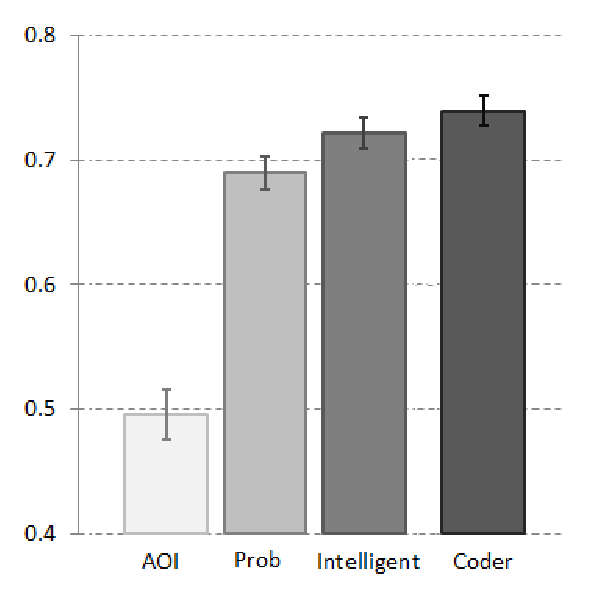
\includegraphics[width=0.6\linewidth]{images/algosComparison.eps}
  \caption{Comparison of different algorithms for analyzing eye tracking data.}
	\label{fig:quantitative}
\end{figure}


\subsubsection{Data collected automatically is relevant and useful}
We use two visual representations and analyses and show that data collected automatically using our instrumentations methods are tightly correlated with the tasks that users had to do. Moreover, we show that such analyses can yield insights into how users perform tasks in an instrumented visualization. We chose this this evaluation method because it essentially provides evidence that the automatic instrumentation approach can be used to solve the inverse problem: an observer or analyst who is unfamiliar to a subject's intentions and worfklows can determine what these are by looking at subjects' visual interest in particular data. 
\textbf{First}, we created heatmap representations from our collected data (FigureX). We listed viewed objects vertically and discretized viewing scores, using averaging, into $250ms$ intervals, which we arranged horizontally. Thus, time is shown horizontally, viewed objects vertically, and intensity of heatmap cells indicate the degree to which an object was viewed at a given moment in time. The viewed objects listed vertically were colored based on their type (movie, actor, director, genre) and could be sorted by either first time they were viewed, amount of viewing activity, or type. 
Figure Xa shows the results for a subject performing the second instance of task 1 (what it is). The heatmap is order by the amount of visual attention that the subject dedicate to each element in the visualization. We notice that the elements at the top of the heatmap are all tightly connected to the task that users were asked to do, which is in accordance to our expectations. Figure Xb shows the same data but ordered by category. We notice that the subject viewed actors early in the task, genres next, followed by directors. Movies were viewed last, except for those directly mentioned in the task, which were viewed throughout the task. This behavior was typical for most of our users in the first task and follows the wording of the task closely: we asked subjects to identify actors, genres, and directors connecting our two movies. 
Figure Xc and Xd shows a subject’s results for one of the instances of task 3, which was significantly less structured than task 1. The heatmap in Xc shows the viewing results order by amount of visual interest, and again we see that the top viewed items are tightly correlated to the task. The heatmap in Figure Xd is sorted by the first time each object was viewed and shows how subjects were moving through different aspects of the analyses, and revisiting them at different moments in time. 
\textbf{Second}, we formalized the relevance of each visual item to a particular task and plot this relevance against the amount of interest that each item attracted, as shown in Figure Y. These plots illustrate the degree to which task relevance impacts the amount that each visual item is tended do by subjects and demonstrate that our instrumentation captures data that is relevant to the tasks that users are performing, rather than noise. 
We formalize the relevance of a visual item to a task as the network minimum distance between that item any item mentioned in the task description.  This definition is not complete as items might be relevant to a task even though they are not directly mentioned in the description.  For instance, items that eventually constitute the subject's answer to the task will elicit more of the subject's attention. Some example of these cases are noticeable in Figure~\ref{fig:RelevanceDiagram}, as points that are much higher on the y-axis then their relevance category's average. Moreover, this definition is particular to the visualization we instrumented.
A few insights can be drawn from analyzing these images. First, even though many items were shown to subjects during their tasks, only a few were viewed for significant periods of time and many were not viewed at all. In fact, the interest in a particular item drops exponentionally with that item's relevance to the task which aligns with knowledge that people's perception is goal-driven~\cite{something} and demonstrates that our instrumentation captures relevant data.  Second, the types of data that users view more are correlated to the task particuliarities as well. For example, task 3 involved movie recommendations and Figure~\ref{fig:RelevanceDiagram}(c) illustrates that genres and directors more viewed significantly more than in task 4 which involved determining the identify of a group of actors who acted in movies together and as such involved primarily the viewing of movies and actors.  




\begin{figure}[!hbt]
  \centering
  \includegraphics[width=0.9\linewidth]{images/RelevanceDiagramTask1.eps}
	\caption*{Relevance Diagram Task 1}
	\includegraphics[width=0.61\linewidth]{images/RelevanceDiagramTask2.eps}
	\caption*{Relevance Diagram Task 2}
	\includegraphics[width=0.71\linewidth]{images/RelevanceDiagramTask3.eps}
	\caption*{Relevance Diagram Task 3}
	\includegraphics[width=\linewidth]{images/RelevanceDiagramTask4.eps}
	\caption*{Relevance Diagram Task 4}
  \captionof{figure}{Relevance Diagram Task 1}
	\label{fig:RelevanceDiagram}
\end{figure}


\begin{figure*}[!hbtp]
  \centering
  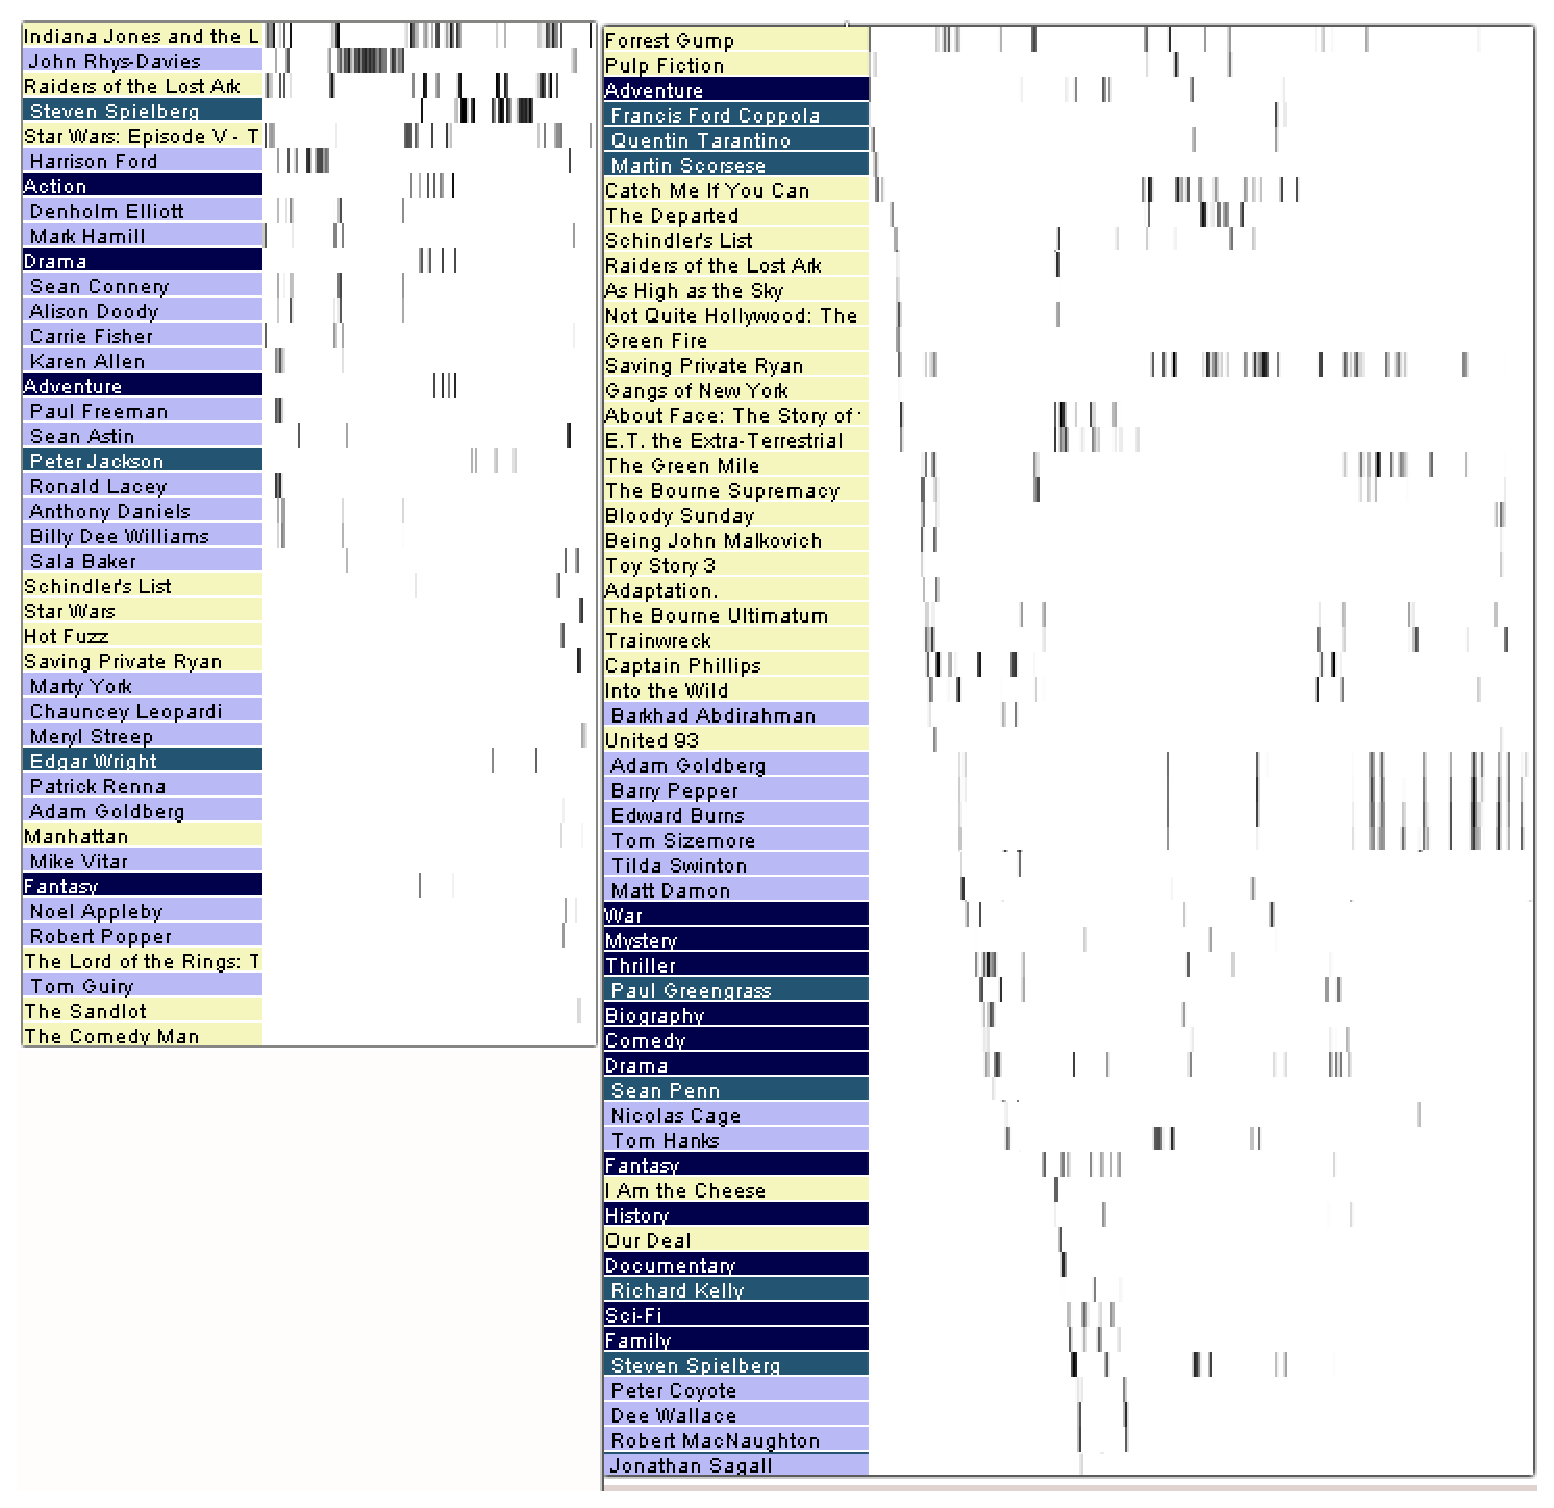
\includegraphics[width=0.75\linewidth]{images/heatmaps.eps}
  \caption{Heatmap views of one subject's activity on two tasks; time, in 500ms increments, are shown horizontally; viewed objects are viewed vertically; cell darkness indicates viewing intensity (black: high; white: low). (Top left) Data for the task 1.ii (see section 4.1); viewed items are ordered by decreasing total amount they were viewed. (Bottom left) Data for the task 1.ii (see section 4.1); viewed items are ordered by category (genre, director, movie, actor). (Right) Data for the task 1.ii (see section 4.1); viewed items are ordered by first time they were seen. 
}
	\label{fig:heatmap}
\end{figure*}


A closer look at the specific data objects listed in the heatmap, as well as their associated viewing activity, removes this concern. In Figure~\ref{fig:heatmap} middle, we restricted the heatmap to showing only data corresponding to the second task subjects completed, which was finding the similarities between the movies ``Raiders of the Lost Ark'' and ``Indiana Jones and the Last Crusade''. The view involved in solving this task contained about $70$ actors, $16$ movies, $11$ directors, and $15$ genres, yet the heatmap reveals that only a small subset of these elements were viewed regularly, and that the more connected the data element was to the task, the more often and intently it was viewed.

Moreover, looking at the data for a single user, sorted by first view, (Figure~\ref{fig:heatmap}) bottom, reveals temporal patterns in how the subject solved the task: they looked at movie titles throughout the task, though predominantly in the beginning, actors in the first half, in a fairly consistent sweep, and directors and genres in the second half. 

\subsubsection{Assumptions about usage patterns hold}
We performed an analysis on common viewing transition patterns in the data that we collected such as how often our subjects transtioned from a genre to an un-highlighted other element vs. to a highlighted other element, or how often subjects transition between a connected element to an uncollected elements. We found that the assumptions described in section X, that users more often transition to connected data elements or to hovered data elements holds. The data is summarized in the highlighted last rows of the panels in Table~\ref{tab:TransitionFromMovie}. 

To this end, we used our collected data but discarded the prediction component, since the prediction component incorporates the very assumptions we try to test and would thus bias the data. We counted transitions between all types of objects to all other types of objects, and we separated transitions to connected objects and to highlighted objects, as seen in the first rows in Table~\ref{tab:TransitionFromMovie}.  For example, after viewing a movie, a user could view either a director, an actor, or genre, each of which can be either connected or connected to the movie, and highlighted or not, or a movie. Since movies are not connected to each other, the user can either view a highlighted or an unhilighted movie in this situation. We note that we skipped transitions to or from empty space and only considered transitions between objects. 

The transition counts between different types of objects are shown in the third row of panels in Table~\ref{tab:TransitionFromMovie}, and their translation into transition probabilities, computed by dividing each transition type by the total number of transitions, is listed in the fourth row. 

However, these numbers could be slightly misleading because they do not take into account the number of objects in each category (e.g., actor, movie, unconnected, connected, highlighted) that a  user could transition to. For example, when transitioning their gaze from a movie to an actor, there are typically many more unconnected and unhighlighted actors to choose from, then there are actors that are either connected to the movie and/or highlighted. As such, it is natural that raw transition counts and probabilities to unconnected and unhighlited  actors should be higher than for other actor transitions. In more concrete example, assume a movie is connected to two actors and there are another eight unconnected items in the view. If there was no transitioning preference for either connected or unconnected items, the probability to jump to a connected item would be 0.2 and 0.8 to jump to an unconnected item. If however, we observe that users jump to one of the two connected items in 50\% of cases, and to unconnected items also in 50\% of cases, then there is clearly a significant biases towards viewing connected items together.


\begin{table}[htbp]
	\centering
		\begin{tabular}{|l|c|}
			\hline
			 \multicolumn{2}{|c|}{Assumed visual and transition weights} \\ \hline
			Movie to unconnected actor & 0.3\\\hline
			Movie to connected actor & 1\\\hline
			Movie to unconnected genre & 0.2\\\hline
			Movie to connected genre & 0.8\\\hline
			Movie to unconnected director & 0.3\\\hline
			Movie to connected director & 1\\\hline
			Any object hovered & 1\\\hline
			Any object not hovered & 0.5\\
			\hline			
		\end{tabular}
	\caption{Transition probabilities in our instrumented visualization (assumed).}
	\label{tab:Transition2}
\end{table}

\begin{table}[htbp]	
	\centering
		\begin{tabular}{|c|c|c|c|c|}
			\hline
			 \multicolumn{2}{ |l| }{Movie to}  &\shortstack{	No. of  \\ Transitions} 	&\shortstack{transition \\ prob.}	&\shortstack{	adjusted \\ transition \\ prob.}\\ \hline
      \multirow{4}{*}{Actor}	&-	&793	&0.076	&0.004	\\	\cline{2-5}
															&H	&147	&0.014	&0.032	\\	\cline{2-5}
															&C	&228	&0.022	&0.019	\\	\cline{2-5}
															&CH	&616	&0.059	&0.089	\\	\hline
				\multirow{2}{*}{Movie}	&-	&5727	&0.548	&0.131	\\	\cline{2-5}
																&H	&1798	&0.172	&0.368	\\	\hline
				\multirow{4}{*}{Director}	&-	&304	&0.029	&0.01	\\	\cline{2-5}
																	&H	&37	&0.004	&0.051	\\	\cline{2-5}
																	&C	&51	&0.005	&0.027	\\	\cline{2-5}
																	&CH	&174	&0.017	&0.135	\\	\hline
				\multirow{4}{*}{Genre}	&-	&193	&0.018	&0.005	\\	\cline{2-5}
																&H	&40	&0.004	&0.027	\\	\cline{2-5}
																&C	&69	&0.007	&0.015	\\	\cline{2-5}
																&CH	&282	&0.027	&0.087	\\	\hline
					\multicolumn{2}{ |l| }{Total}	&10459	&1	&1	\\		
				\hline
		\end{tabular}		
		\caption*{(a)Transitions from Movies}\smallskip
		
		\begin{tabular}{|c|c|c|c|c|}
			\hline
			 \multicolumn{2}{ |l| }{Actor to}  &\shortstack{	No. of  \\ Transitions} 	&\shortstack{transition \\ prob.}	&\shortstack{	adjusted \\ transition \\ prob.}\\ \hline
						 \multirow{2}{*}{Actor}	&-	&4711	&0.533	&0.032	\\	\cline{2-5}
																		&H	&2164	&0.245	&0.372	\\	\hline
							\multirow{4}{*}{Movie}	&-	&839	&0.095	&0.031	\\	\cline{2-5}
																			&H	&213	&0.024	&0.113	\\	\cline{2-5}
																			&C	&386	&0.044	&0.157	\\	\cline{2-5}
																			&CH	&352	&0.04	&0.236	\\	\hline
							\multirow{2}{*}{Director}	&-	&68	&0.008	&0.003	\\	\cline{2-5}
																				&H	&29	&0.003	&0.034	\\	\hline
							\multirow{2}{*}{Genre}	&-	&43	&0.005	&0.002	\\	\cline{2-5}
																			&H	&39	&0.004	&0.02	\\	\hline
								\multicolumn{2}{ |l| }{Total}	&8844	&1	&1	\\	
	\hline

		\end{tabular}
	\caption*{(b)Transitions from Actors}\smallskip
	\begin{tabular}{|c|c|c|c|c|}
			\hline
			 \multicolumn{2}{ |l| }{Director to}  &\shortstack{	No. of  \\ Transitions} 	&\shortstack{transition \\ prob.}	&\shortstack{	adjusted \\ transition \\ prob.}\\ \hline
       \multirow{2}{*}{Actor}	&-	&71	&0.042	&0.001	\\	\cline{2-5}
															&H	&24	&0.014	&0.011	\\	\hline
			\multirow{4}{*}{Movie}	&-	&271	&0.162	&0.031	\\	\cline{2-5}
														&H	&55	&0.033	&0.121	\\	\cline{2-5}
														&C	&130	&0.077	&0.108	\\	\cline{2-5}
														&CH	&93	&0.055	&0.139	\\	\hline
			\multirow{2}{*}{Director}	&-	&384	&0.229	&0.054	\\	\cline{2-5}
																&H	&160	&0.095	&0.299	\\	\hline
			\multirow{2}{*}{Genre}	&-	&256	&0.153	&0.026	\\	\cline{2-5}
															&H	&234	&0.139	&0.211	\\	\hline
				\multicolumn{2}{ |l| }{Total}	&1678	&1	&1	\\	
				\hline
		\end{tabular}
		\caption*{(c)Transitions from Director}\smallskip
		\begin{tabular}{|c|c|c|c|c|}
			\hline
			 \multicolumn{2}{ |l| }{Genre to}  &\shortstack{	No. of  \\ Transitions} 	&\shortstack{transition \\ prob.}	&\shortstack{	adjusted \\ transition \\ prob.}\\ \hline
       \multirow{2}{*}{Actor}	&-	&61	&0.03	&0	\\	\cline{2-5}
															&H	&32	&0.016	&0.011	\\	\hline
				\multirow{4}{*}{Movie}	&-	&229	&0.113	&0.012	\\	\cline{2-5}
																&H	&46	&0.023	&0.077	\\	\cline{2-5}
																&C	&172	&0.085	&0.024	\\	\cline{2-5}
																&CH	&138	&0.068	&0.135	\\	\hline
				\multirow{2}{*}{Director}	&-	&282	&0.139	&0.015	\\	\cline{2-5}
																	&H	&195	&0.096	&0.383	\\	\hline
				\multirow{2}{*}{Genre}	&-	&348	&0.172	&0.013	\\	\cline{2-5}
																&H	&526	&0.259	&0.328	\\	\hline
					\multicolumn{2}{ |l| }{Total}	&2029	&1	&1	\\	
			\hline
		\end{tabular}
		\caption*{(d)Transitions from Genres}\smallskip
	\captionof{table}{Transitions from Movies}
	\label{tab:TransitionFromMovie}
\end{table}

